\section{DiffuCoder}
\label{sec:diffucoder}
To build a strong base model for RL training, we follow common practices in LLM training and train our DiffuCoder model on a large-scale corpus~\citep{lozhkov2024starcoder} with multiple training stages; the pipeline is illustrated in Figure~\ref{fig:pipeline}.
We first conduct adaptation pre-training similar to the process followed by Dream~\citep{dream2025}. 
Mid-training~\citep{wang2025octothinker} connects the pre-training and post-training stages, plays the role of an annealing phase as in OpenCoder~\citep{huang2024opencoder}, and has proven effective.
% \citet{wang2025octothinker} also highlight the importance of mid-training during RL scaling of AR reasoning models.
This is followed by an instruction tuning stage to enhance the model's capability of following instructions. Finally, for post-training, we employ a novel \textbf{coupled-GRPO} method (introduced in \S\ref{sec:grpo}) to further enhance the model's pass@1 coding capabilities.
% \subsection{Experiment Setup}
\begin{figure}
    \centering
    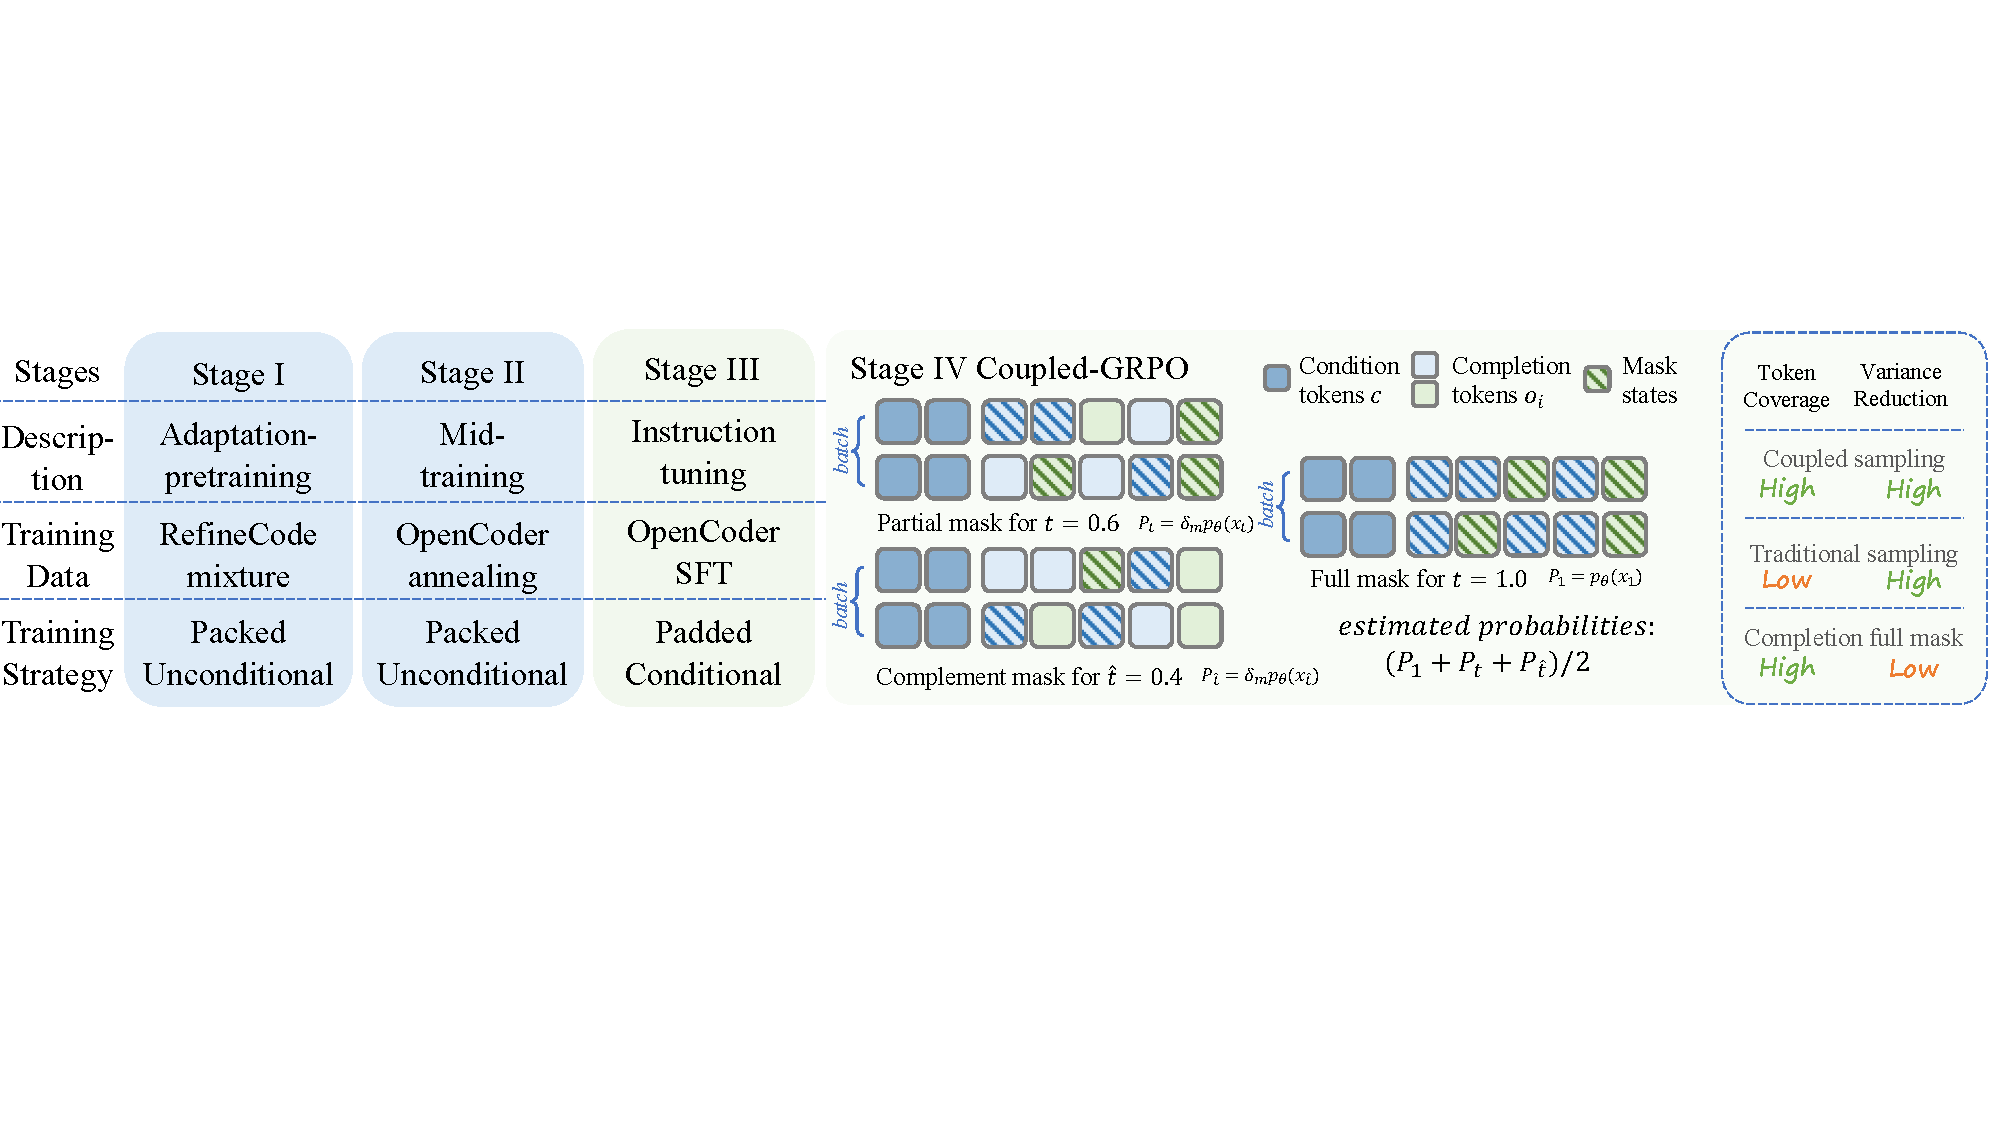
\includegraphics[width=1\linewidth]{fig/coupled-grpo.pdf}
    \caption{Pipeline of DiffuCoder training stages and an illustration of the coupled-GRPO algorithm. We sample complementary mask matrices for the same batch, so the coupling probability matrices can be merged into one full matrix. Coupled sampling reduces probability estimation variance while maintaining full token coverage, where each token is sampled exactly the same number of times.}
    \label{fig:pipeline}
\end{figure}
\label{sec:exp}
\paragraph{Training} We adapt our model from Qwen-2.5-Coder~\citep{hui2024qwen2} as the base model to perform continual pre-training using the adaptation approach from~\citet{gong2025scaling}.
During this pre-training, we use a 400B-token code pre-training corpus from 
RefineCode~\citep{huang2024opencoder}
and Stackv2~\citep{lozhkov2024starcoder}. We adopt the code-to-text ratio suggested in Qwen-2.5-Coder and OpenCoder~\citep{huang2024opencoder}. 
We use 16B tokens of annealing code data during mid-training and 436K SFT samples during instruction tuning, both from OpenCoder~\citep{huang2024opencoder}. For RL training, we select 21K hard samples from Acecoder-87K~\citep{zeng2025acecoder} with verifiable test cases. We build our post-training method upon the Open-R1\footnote{\url{https://github.com/huggingface/open-r1}} codebase. All experiments are conducted on 8 to 10 nodes, each with 8 H100 GPUs. 
We observed that training with 700B tokens in Stage 1 led to worse performance than using only 65B tokens on the downstream validation sets. Therefore, we perform early stopping for Stage 1, training on 65B tokens. In Stage 2, we train for 4 epochs, totaling 65B tokens with repeats, as the mid-training data is less noisy. 
More details are listed in Appx.~\ref{appx:exp}.
\paragraph{Evaluation}
Our evaluation environments are built on three code benchmarks and their variants: HumanEval~\citep{chen2021evaluating}, MBPP~\citep{austin2021program}, EvalPlus (HumanEval+ and MBPP+;~\citealt{liu2023your}), and BigCodeBench~\citep{zhuo2024bigcodebench} with full and hard subsets in completion (C) and instruction (I) query types. 
These benchmarks, with Python as the coding language, provide a diverse set of coding tasks for assessing code correctness and quality.
% \subsection{DiffuCoder}
\paragraph{Performance} We compare our models with AR code LLMs, including Qwen2.5-Coder-7B~\citep{hui2024qwen2}, OpenCoder-8B~\citep{huang2024opencoder}; general dLLMs, such as Dream-7B~\citep{dream2025} and LLaDA-8B~\citep{li2025llada}; and commercial models, such as GPT-4o\footnote{\url{https://openai.com/index/gpt-4o-system-card/}}, Mercury\footnote{\url{https://chat.inceptionlabs.ai/}}, and Gemini Diffusion\footnote{\url{https://deepmind.google/models/gemini-diffusion/}}. 
As shown in Table~\ref{tab:maintab}, DiffuCoder, after being continually trained on 130B code tokens (Stages 1 and 2), achieves performance on par with Qwen2.5-Coder and OpenCoder. 
However, all dLLMs show only marginal improvement over their base models after instruction tuning, especially when compared to Qwen2.5-Coder+SFT, which achieves large improvements from being instruct-tuned on the same data. 

This improvement gap between AR and dLLMs at the instruction-tuning stage motivates us to explore RL-based post-training methods (\S\ref{sec:grpo}). 
Previous RL approaches for diffusion models~\citep{zhao2025d1,yang2025mmada} rely heavily on semi-AR decoding, which deviates from diffusion's global nature. 
To design RL methods aligned with diffusion's non-autoregressive principle, we first analyze the intrinsic decoding behavior of dLLMs and their differences from AR models in \S\ref{sec:understanding}.

\begin{table}[t]
    \centering
    \small
    \setlength{\tabcolsep}{4pt} 
    \caption{Benchmark coding capacities of LLMs and dLLMs in 7/8B scale. Different shaded colors indicates different generation paradigms (pink for AR, yellow for diffusion). $^*$ denotes that the results are collected from public reports instead of evaluating by ourselves. In our evaluation settings, we compute EvalPlus as the average of HE+ and MBPP+. We show the absolute score change (±) of each instruct model relative to its base. Scores are bolded when our model outperforms LLMs specialized for code (excluding LLaDA or Dream).}
    \begin{tabular}{@{} l ll ll l ll l @{}}
        \toprule
        \multirow{2}{*}{\textbf{Model}}
            & \multicolumn{2}{c}{HumanEval}
            & \multicolumn{2}{c}{MBPP}
            & \multirow{2}{*}{EvalPlus}
            & \multicolumn{2}{c}{BigCodeBench (C)} 
            & \multirow{2}{*}{Avg.}\\
        \cmidrule(lr){2-3} \cmidrule(lr){4-5} \cmidrule(lr){7-8}
            & -   & Plus
            & -   & Plus
            & 
            & \multicolumn{1}{c}{Full} & \multicolumn{1}{c}{Hard} & \\
        \midrule
        \multicolumn{9}{c}{\textbf{Base Models}} \\
        \midrule
        \cellcolor{lightRed!12}Qwen2.5-Coder      & 61.6  & 51.8  & 75.9  & 61.4  & 56.6  & 46.1  & 16.2  &52.2 \\
        \cellcolor{lightRed!12}OpenCoder$^*$      & 66.5  & 63.4  & 79.9  & 70.4  & 66.9  & 40.5  & 9.5  & 55.0 \\
        \cellcolor{lightYellow!12}LLaDA         & 35.4  & 30.5  & 50.1  & 42.1  & 36.3  & 18.9  & 4.1  & 30.2 \\
        \cellcolor{lightYellow!12}Dream         & 56.7  & 50.0  & 68.7  & 57.4  & 53.7  & 23.6  & 4.1  & 43.4\\
        \cellcolor{lightYellow!12}DiffuCoder            & \textbf{67.1}  & \textbf{60.4}  & 74.2  & 60.9  & \textbf{60.6}  & 40.2  & \textbf{12.8}  & \textbf{52.6} \\
        \midrule
        \multicolumn{9}{c}{\textbf{Instruct Models}} \\
        \midrule
        \cellcolor{lightRed!12}Qwen2.5-Coder-Instruct & 90.2  & 85.4  & 83.9  & 72.0  & 78.7  & 50.7  & 21.6  & 67.3 \\
        \cellcolor{lightRed!12}Qwen2.5-Coder+SFT      
        & 82.9{\tiny\textcolor{ForestGreen}{+21.3}}  
        & 75.6{\tiny\textcolor{ForestGreen}{+23.8}}  
        & 80.1{\tiny\textcolor{ForestGreen}{+4.2}}  
        & 66.1{\tiny\textcolor{ForestGreen}{+4.7}}  
        & 70.9{\tiny\textcolor{ForestGreen}{+14.3}}  
        & 46.9{\tiny\textcolor{ForestGreen}{+0.8}}  
        & 16.2{\tiny\textcolor{red}{–0.0}}  
        & 61.3{\tiny\textcolor{ForestGreen}{+9.1}} \\
        \cellcolor{lightRed!12}OpenCoder-Instruct$^*$      
        & 83.5{\tiny\textcolor{ForestGreen}{+17.0}}  
        & 78.7{\tiny\textcolor{ForestGreen}{+15.3}}  
        & 79.1{\tiny\textcolor{red}{–0.8}}  
        & 69.0{\tiny\textcolor{red}{–1.4}}  
        & 73.9{\tiny\textcolor{ForestGreen}{+7.0}}  
        & 40.3{\tiny\textcolor{red}{–0.2}}  
        & 16.9{\tiny\textcolor{ForestGreen}{+7.4}}  
        & 61.3{\tiny\textcolor{ForestGreen}{+6.3}} \\
        \cellcolor{lightYellow!12}LLaDA-Instruct        
        & 35.4{\tiny\textcolor{red}{–0.0}}  
        & 31.7{\tiny\textcolor{ForestGreen}{+1.2}}  
        & 31.5{\tiny\textcolor{red}{–18.6}}  
        & 28.6{\tiny\textcolor{red}{–13.5}}  
        & 30.2{\tiny\textcolor{red}{–6.1}}  
        & 16.5{\tiny\textcolor{red}{–2.4}}  
        & 2.7{\tiny\textcolor{red}{–1.4}}  
        & 24.4{\tiny\textcolor{red}{–5.8}} \\
    \cellcolor{lightYellow!12}Dream-Instruct        
        & 57.9{\tiny\textcolor{ForestGreen}{+1.2}}  
        & 53.7{\tiny\textcolor{ForestGreen}{+3.7}}  
        & 68.3{\tiny\textcolor{red}{–0.4}}  
        & 56.1{\tiny\textcolor{red}{–1.3}}  
        & 54.9{\tiny\textcolor{ForestGreen}{+1.2}}  
        & 10.6{\tiny\textcolor{red}{–13.0}}  
        & 0.7{\tiny\textcolor{red}{–3.4}}  
        & 41.2{\tiny\textcolor{red}{–2.2}} \\
    \cellcolor{lightYellow!12}DiffuCoder-Instruct   
        & 72.0{\tiny\textcolor{ForestGreen}{+4.9}}  
        & 65.2{\tiny\textcolor{ForestGreen}{+4.8}}  
        & 75.1{\tiny\textcolor{ForestGreen}{+0.9}}  
        & 61.9{\tiny\textcolor{ForestGreen}{+1.0}}  
        & 63.6{\tiny\textcolor{ForestGreen}{+3.0}}  
        & 35.7{\tiny\textcolor{red}{–4.5}}  
        & 12.2{\tiny\textcolor{red}{–0.6}}  
        & 53.7{\tiny\textcolor{ForestGreen}{+1.1}} \\
    \cellcolor{lightYellow!12}\quad + coupled-GRPO   
        & 73.2{\tiny\textcolor{ForestGreen}{+6.1}}  
        & 68.3{\tiny\textcolor{ForestGreen}{+7.9}}  
        & \textbf{78.6}{\tiny\textcolor{ForestGreen}{+4.4}}  
        & 67.5{\tiny\textcolor{ForestGreen}{+6.6}}  
        & 67.9{\tiny\textcolor{ForestGreen}{+7.3}}  
        & 40.4{\tiny\textcolor{ForestGreen}{+0.2}}  
        & 10.8{\tiny\textcolor{red}{–2.0}}  
        & 56.5{\tiny\textcolor{ForestGreen}{+3.9}} \\
        \midrule
        \multicolumn{9}{c}{\textbf{Commercial Models}} \\
        \midrule
        \cellcolor{lightRed!12}GPT 4o$^*$             & 90.2  & –     & 82.2  & –     & 82.4  & 49.9  & –   & – \\
        \cellcolor{lightYellow!12}Mercury$^*$             & 90.0    & –     & 77.1  & –     & 80.4  & 45.5  & –   &–  \\
        \cellcolor{lightYellow!12}Gemini Diffusion$^*$            & 89.6    & –     & 76.0  & –     & –  & 45.4  & –   & – \\
        \bottomrule
    \end{tabular}
    \label{tab:maintab}
\end{table}


\section{Understanding Mask Diffusion Models based on DiffuCoder}
\label{sec:understanding}
Current dLLMs such as LLaDA~\citep{nie2024scaling} and Dream rely on low-confidence remasking decoding strategies~\citep{maskgit}, and LLaDA achieves improved performance on certain tasks using semi-AR decoding methods (\textit{i.e.}, block diffusion decoding; see~\citealp{arriola2025block}). Another common practice among dLLMs is to set the number of diffusion timesteps equal to the sequence length, effectively resorting to token-by-token generation to enhance performance. Given this context, we introduce local and global \emph{autoregressive-ness} (AR-ness) metrics to systematically investigate the decoding order of dLLMs. Specifically, our analysis aims to demystify: (1) how dLLMs' decoding patterns differ from those of AR models; (2) how data modality (\textit{e.g.}, code or math) influences model behavior; and (3) how AR-ness evolves across different training stages.

\subsection{Autoregressive-ness in Generation}
\label{sec:metricdefine}
\begin{figure}[h]
  \centering
  \begin{subfigure}[c]{0.655\textwidth}
    \centering
    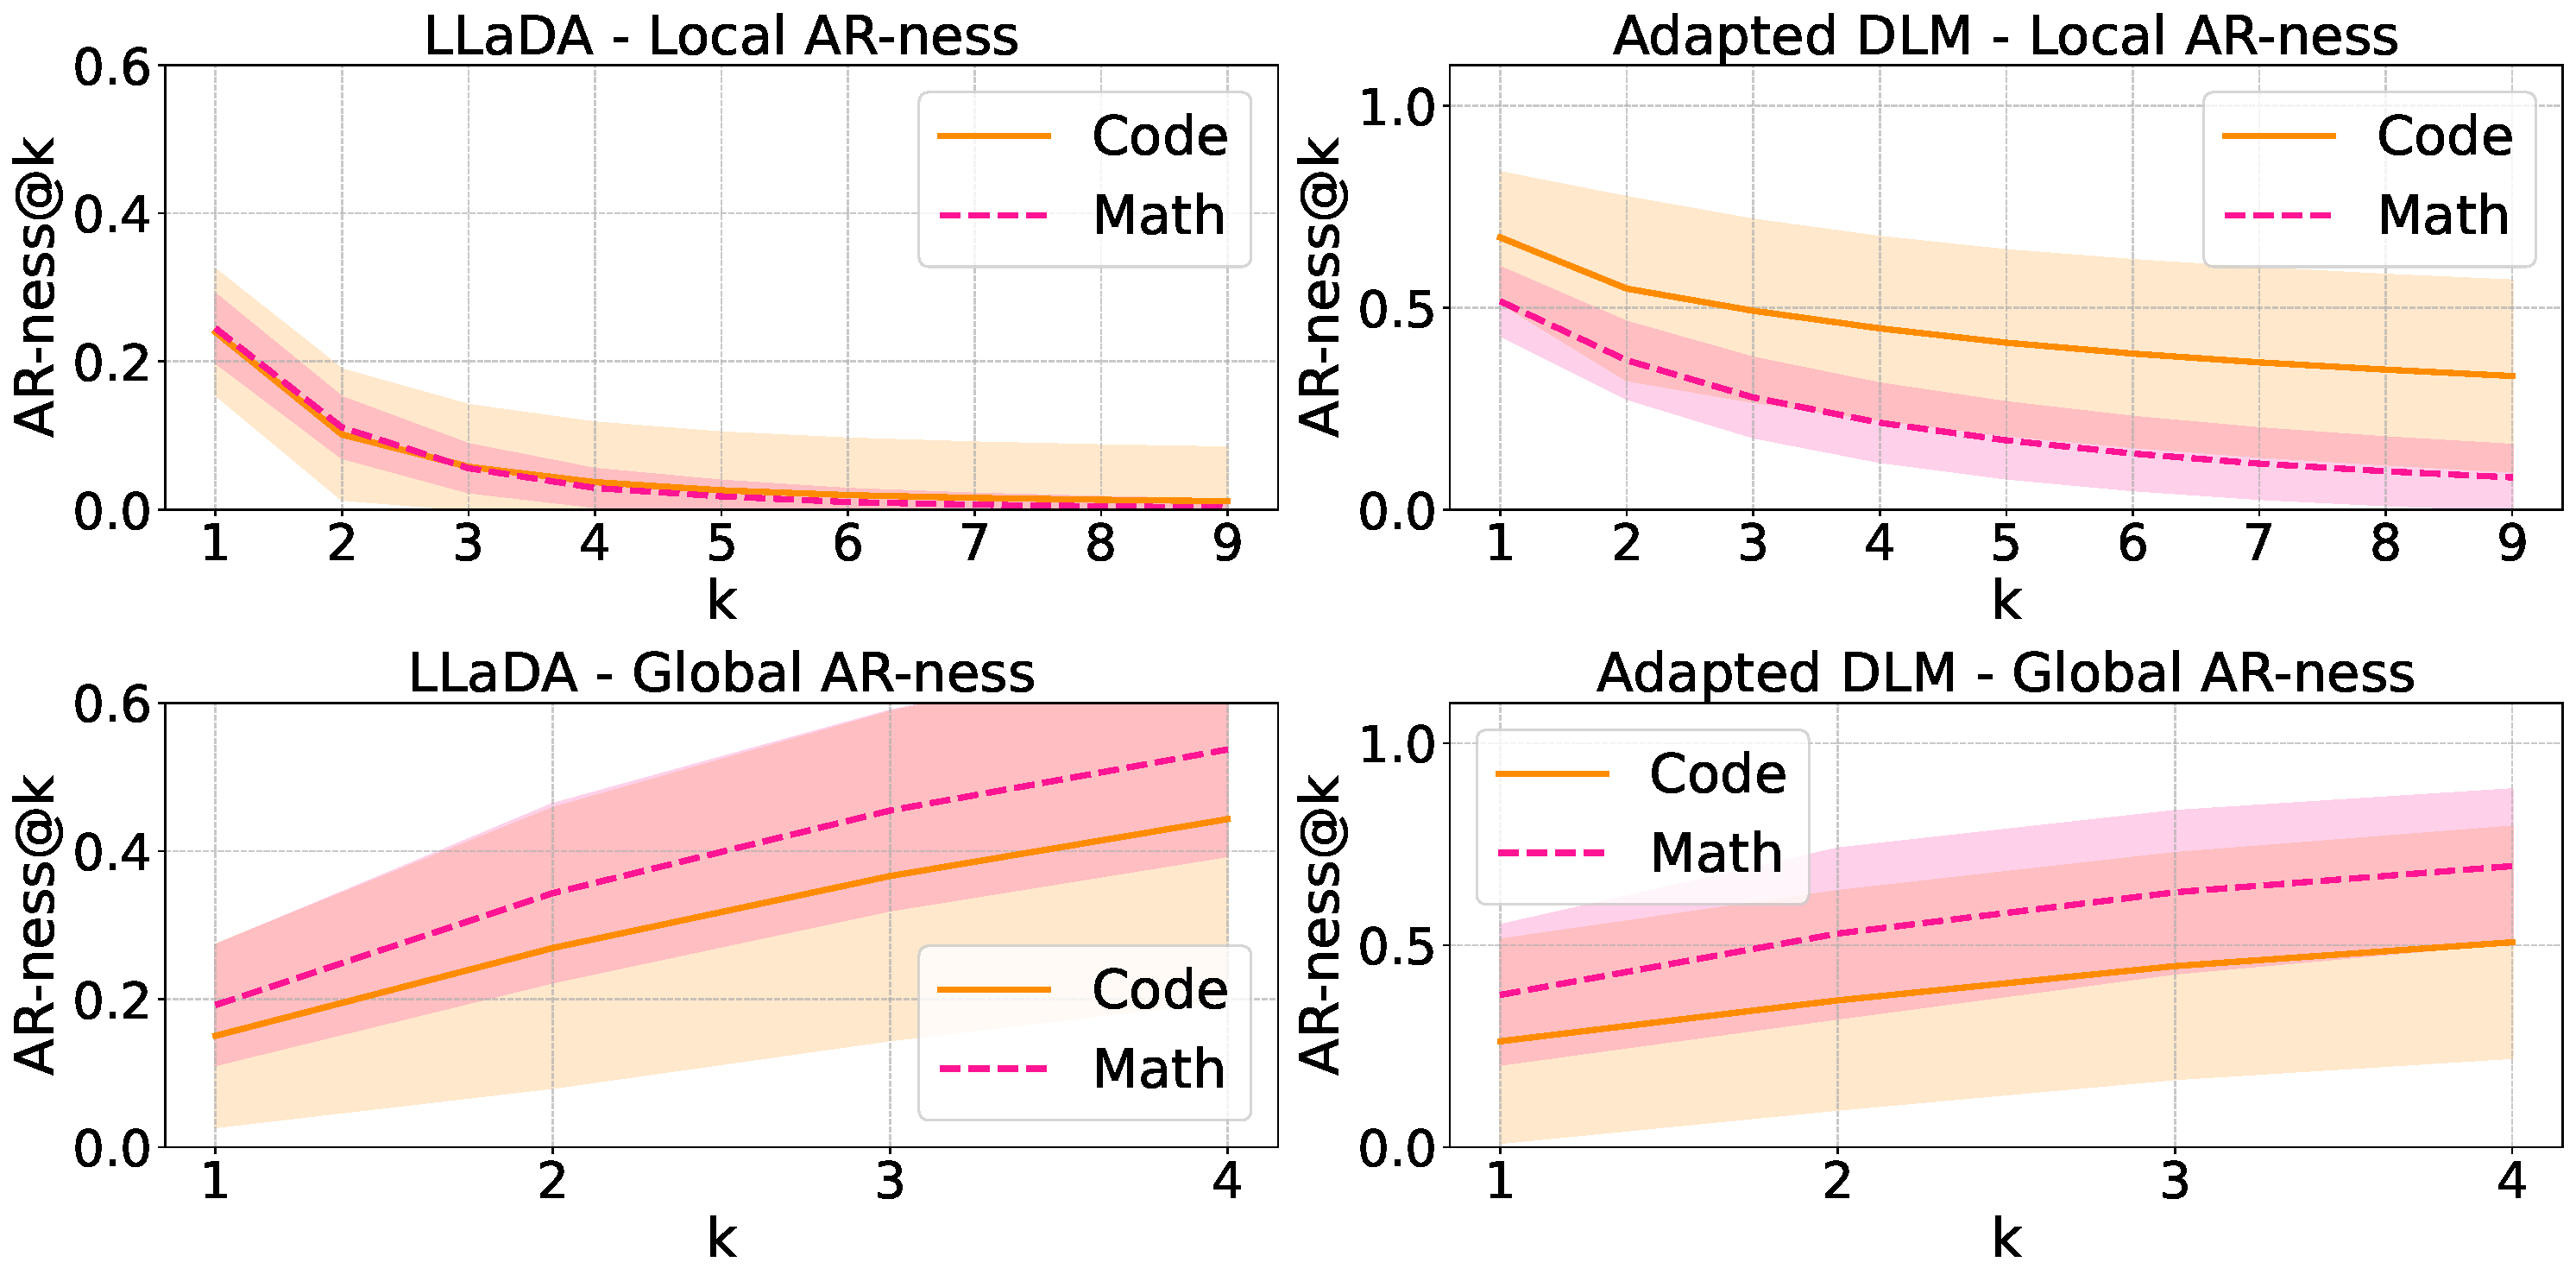
\includegraphics[width=\linewidth]{fig/ntpr-analysis-causality.pdf}
  \end{subfigure}
  \hfill
  \begin{subfigure}[c]{0.335\textwidth}
    \centering
    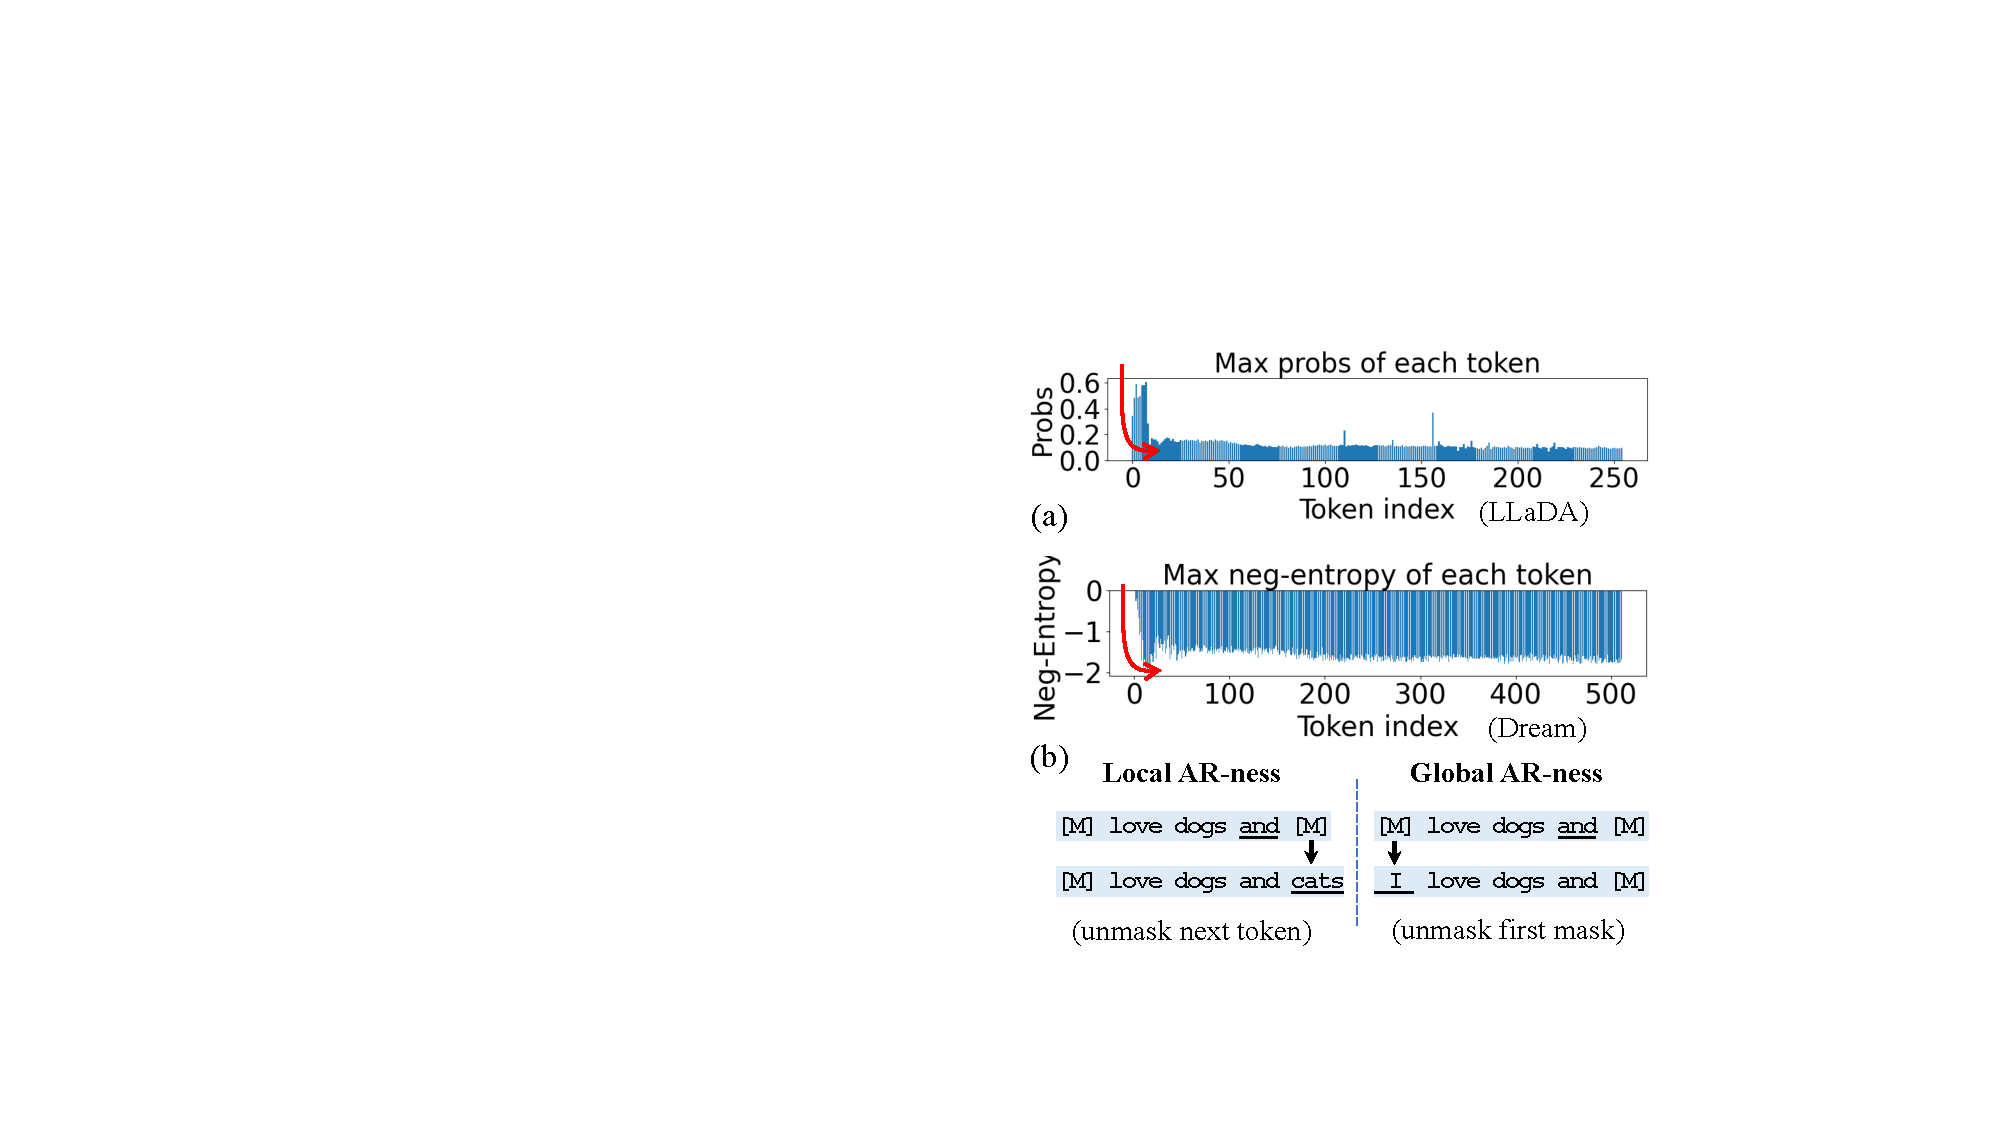
\includegraphics[width=\linewidth]{fig/entropy2.pdf}
  \end{subfigure}
  \caption{\textbf{Left}: Local and global AR-ness across different models and data modalities. Adapted dLLM refers to Dream for the math task and DiffuCoder (Stage 1 trained with 65B tokens) for the code task. \textbf{Right}: (a) Confidence score for each position in the dLLM's first forward decoding step. (b) Local \textit{AR-ness@k}: the fraction of decoding steps where the newly unmasked token, together with the $k$ immediately preceding predicted tokens, forms a strictly increasing consecutive sequence, at $k=1$ for next-token prediction. Global \textit{AR-ness@k}: the fraction of decoding steps where the model chooses to unmask one of the earliest $k$ positions among all remaining masked tokens.}
    \label{fig:causal analysis} 
\end{figure}

\begin{figure}[th]
  \centering
  \begin{subfigure}[c]{0.495\textwidth}
    \centering
    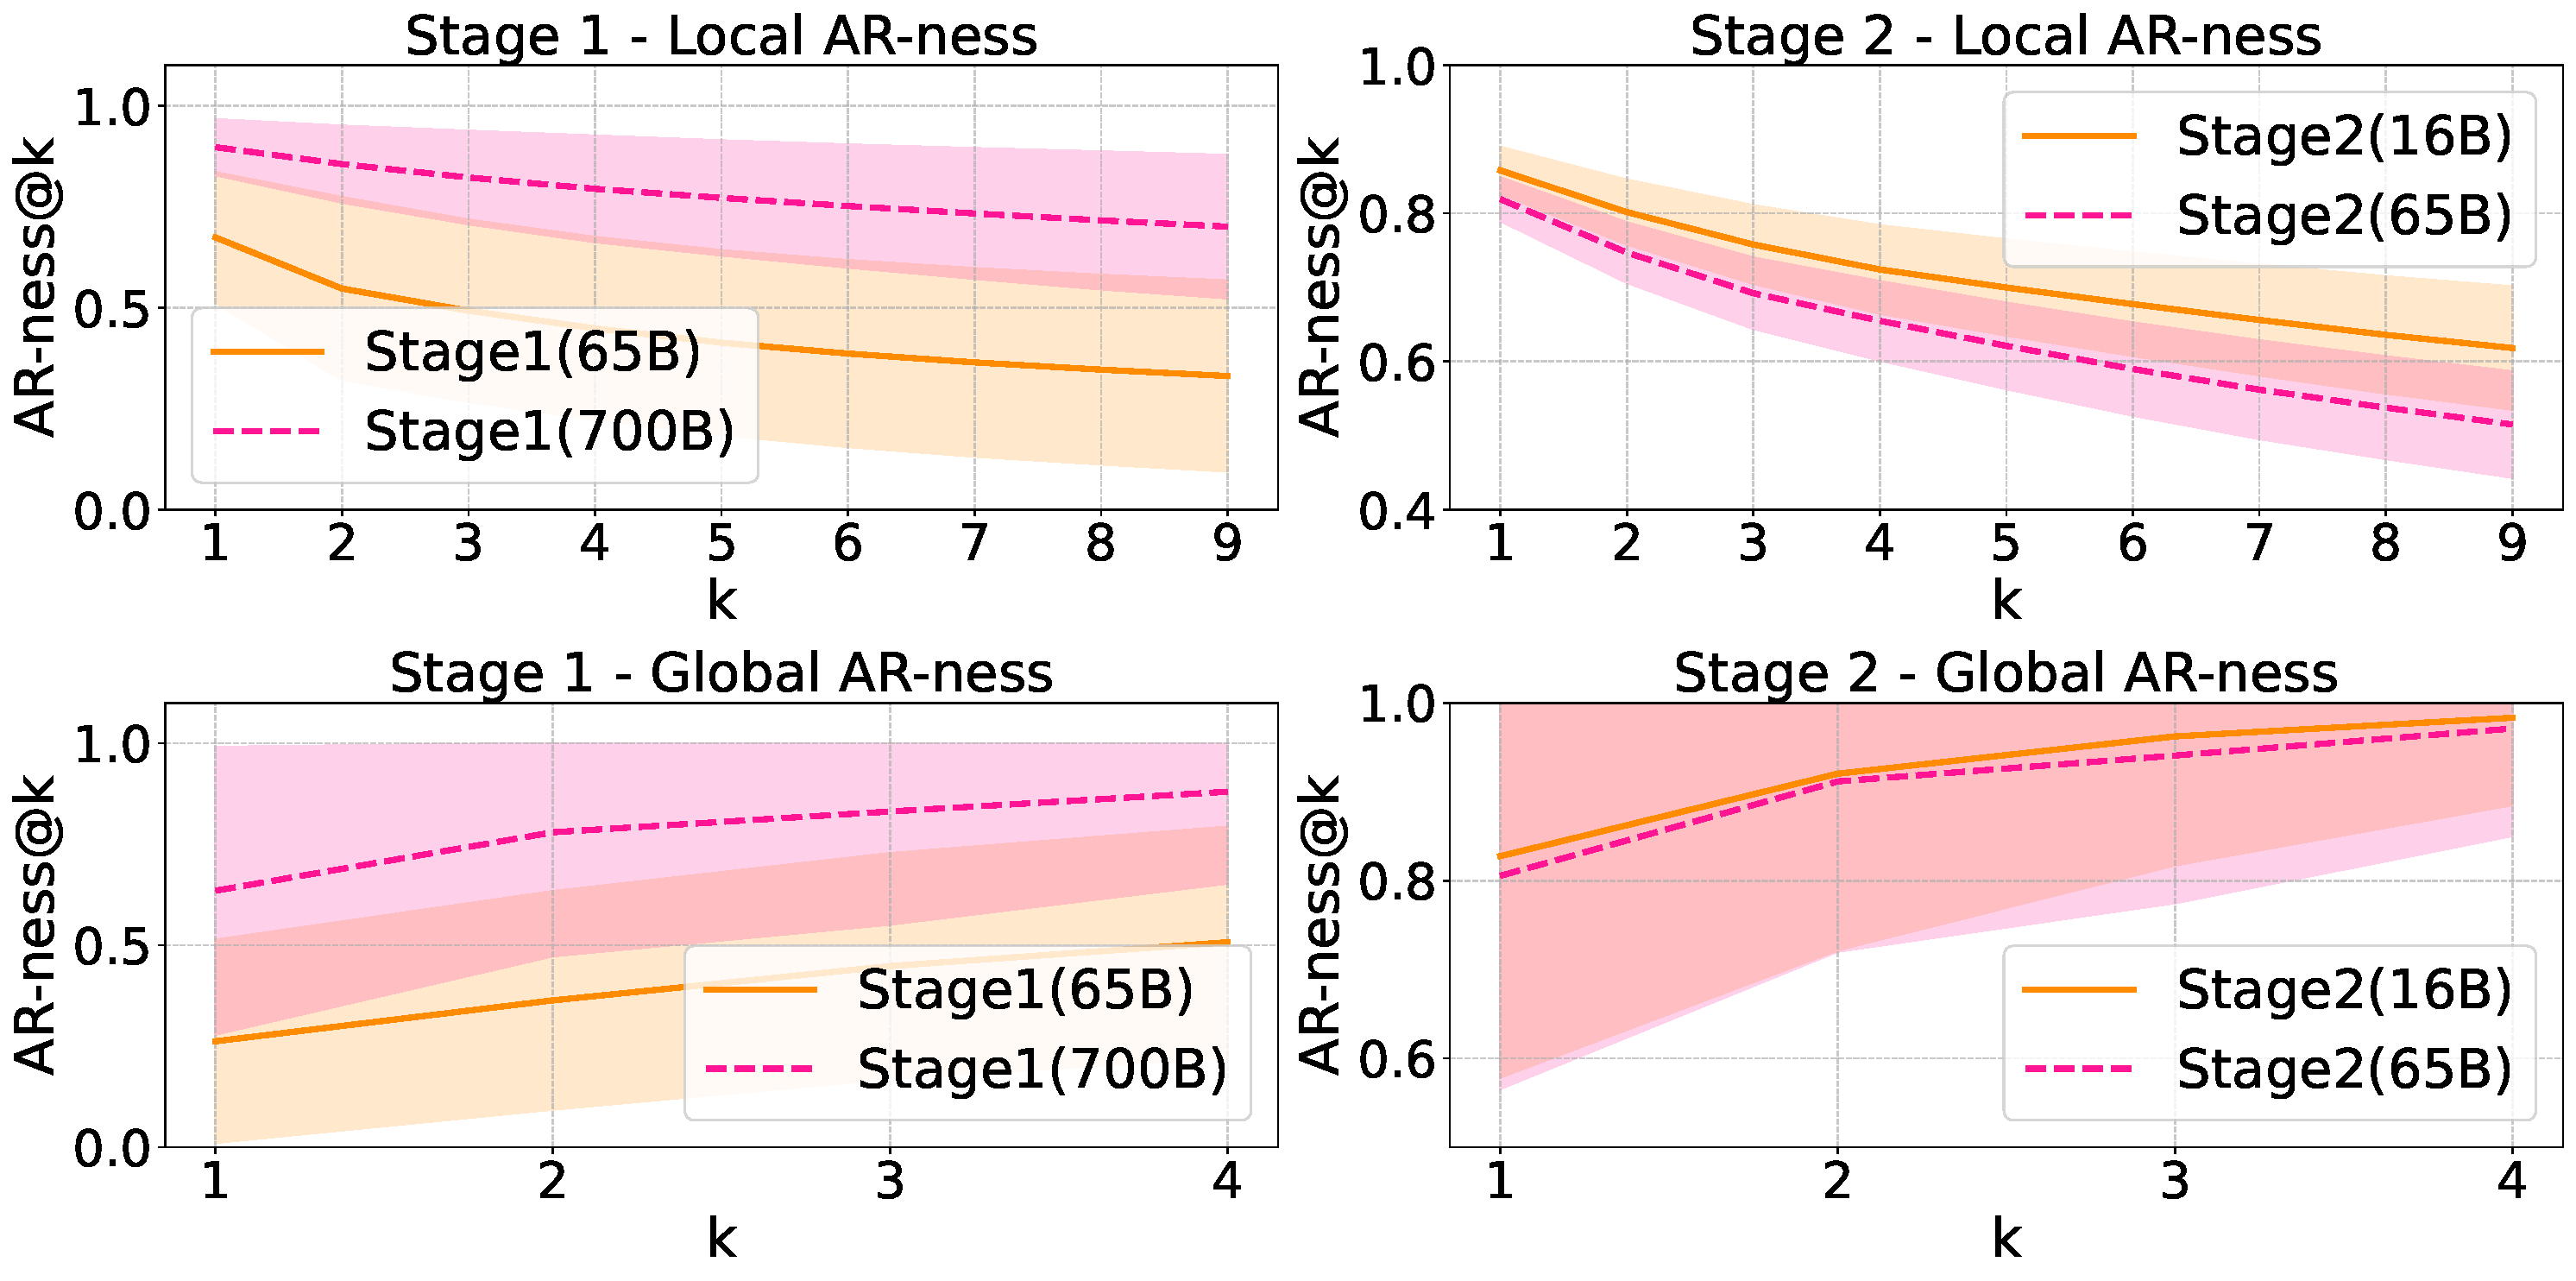
\includegraphics[width=\linewidth]{fig/ntpr-analysis-stages.pdf}
  \end{subfigure}
  \hfill
  \begin{subfigure}[c]{0.495\textwidth}
    \centering
    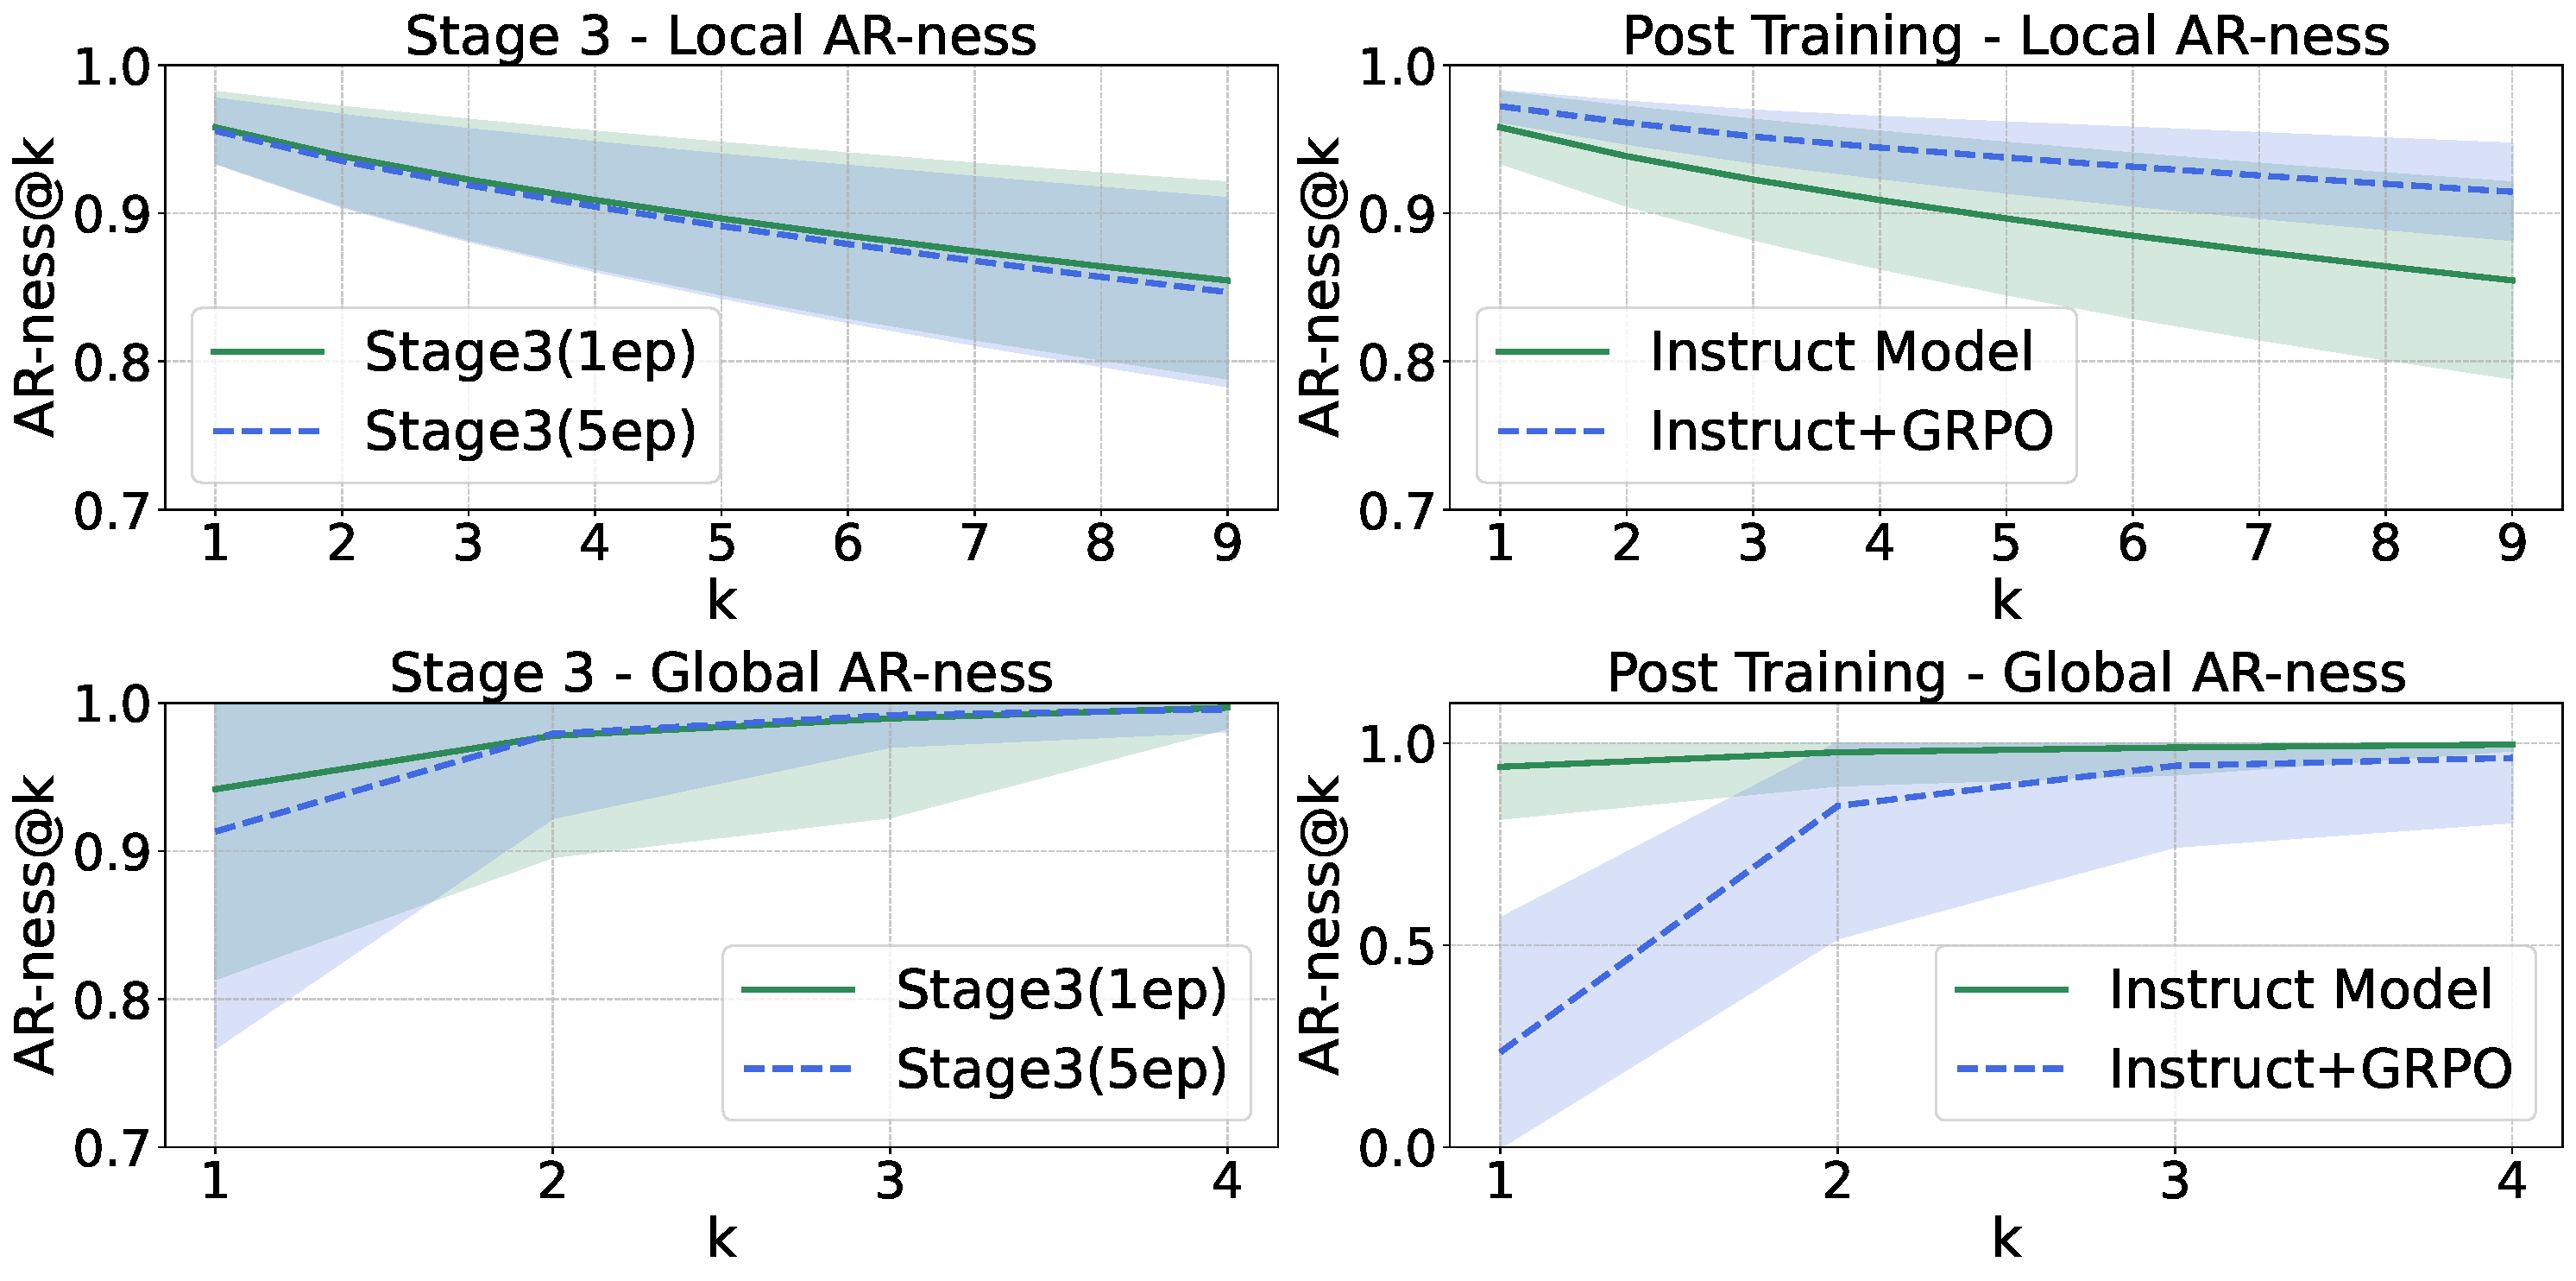
\includegraphics[width=\linewidth]{fig/ntpr-analysis-stages2.pdf}
  \end{subfigure}
  \caption{AR-ness drifts on different training stages. \textbf{Left}: adaptation pre-training stage and mid-training stage. \textbf{Right}: instruction tuning and RL post-training stage.}
    \label{fig:causal-stages} 
\end{figure}

In standard AR decoding, the model generates tokens in strict left‐to‐right order, ensuring strong sequential coherence. 
However, diffusion-based decoding may choose to recover \mask out of order. 
Therefore, we introduce two metrics to quantify how the unmasking schedule of a diffusion model resembles an AR pattern, including (i) ``next token'' pattern and (ii) ``left first'' pattern. 

\paragraph{Local: Consecutive Next‐Token Prediction}
\emph{Local AR-ness@\(k\)} is computed by the ratio of predicted sequence matching the pattern of next token prediction within range $k$. 
If all tokens in $k$-length span are immediate successors of the previously generated token, we count this span as casual. 
Local AR-ness decays as \(k\) grows, as it is harder to maintain longer consecutive spans.

\paragraph{Global: Earliest Mask Selection}
In step \(t\), if the predicted token lies in the first $k$ masked positions, the global AR-ness is scored. \emph{Global AR-ness@\(k\)} is the averaged ratio for each $t$, and it measures the tendency to always unmask the earliest remaining token, capturing a left-to-right filling strategy. 
This ratio grows with \(k\), since the criterion becomes easier to satisfy as more early positions are allowed.
For the two metrics, the higher value indicates that the generation is more autoregressive.
Detailed formulations are listed in Appx.~\ref{appx:Causality}.

\subsection{Decoding Analysis}
\label{sec:analysis}
We conduct AR-ness comparisons during conditional generation between: (1) different dLLMs, including LLaDA trained from scratch and Dream or DiffuCoder adapted from AR LLMs; (2) different data modalities, including math and code; and (3) different training stages of DiffuCoder. 
All inference settings are based on the low-confidence remasking strategy~\citep{maskgit} with the same sequence length and diffusion timesteps ($512$). Math is evaluated on GSM8K using 8-shots~\citep{cobbe2021training}, and code is evaluated using zero-shot HumanEval.

\paragraph{How do dLLMs decode differently from AR models?}
For AR decoding, both local and global AR-ness are identically equal to $1$ (\textit{i.e.}, 100\% AR). 
In contrast, as illustrated in Figure~\ref{fig:causal analysis}, dLLMs do not always decode in a purely AR manner. 
A significant fraction of tokens in dLLM decoding are recovered from neither the leftmost masked token nor the next token. 
This observation indicates that dLLMs adopt a more flexible decoding order compared to regular AR models.
Nevertheless, both local and global AR-ness are closer to $1$ than $0$, demonstrating that text data inherently exhibit some AR structure, which diffusion-based LMs, regardless of whether they are trained from scratch or adapted from AR models, naturally capture. 
Empirically, adapted dLLMs tend to exhibit stronger AR-ness than those trained from scratch. 
This is because they inherit the left-to-right token dependencies from the original AR training. 
Lower AR-ness opens up additional opportunities for parallel generation by breaking this dependency (Appx.~\ref{sec:appx:decodet}). 
Higher AR-ness can also be beneficial; for example, LLaDA often needs to resort to semi-AR (block-wise decoding;~\citealp{arriola2025block}) generation to achieve higher overall performance. 
In that setting, the block decoder explicitly reintroduces causal bias into the generation process. In DiffuCoder, we argue that the model can decide how causal it is during generation by itself.
\paragraph{How do different data modalities affect the decoding paradigm?} 
According to Figure~\ref{fig:causal analysis}, although math and code decoding exhibit different degrees of local AR-ness, a consistent finding is that code generation has a lower mean and higher variance in global AR-ness. 
This indicates that when generating code, the model tends to produce later tokens first, leaving some early masked tokens un-recovered until much later (Appx.~\ref{sec:appx:samples}). 
The reason might be that mathematical text is essentially sequential and usually requires left-to-right computation, whereas code has an intrinsic structure. 
Consequently, the model often plans token generation more globally, much like a programmer jumping back and forth through code to refine a code implementation.
\paragraph{How does AR-ness change at different training stages?}
In Figure~\ref{fig:causal-stages} (Stage 1), after training with 65B tokens, we already observe a relatively low AR-ness. 
However, when we extend the training to 700B tokens, AR-ness increases while overall performance drops (see the table in Appx.~\ref{appx:exp}). 
We suspect that the quality of the pre-training data limits performance. 
Consequently, we choose the Stage 1 65B model as the starting point for Stage 2.
During mid-training (Stage 2) and instruction tuning (Stage 3), on the first epoch of high-quality data, the model learns a high causal bias.
As it sees more tokens, however, task performance improves (Appx.~\ref{appx:exp}), while the measured AR-ness starts to decline. 
This pattern implies that after the first epoch, dLLMs begin to capture dependencies beyond a pure AR order. 
After GRPO training, the model's global AR-ness also decreases and meanwhile shows less of a performance drop when decoding in half as many steps (Figure~\ref{fig:teaser}(c); Appx.~\ref{sec:appx:decodet}).

\paragraph{Entropy Sink} 
When dLLMs perform conditional generation, the first diffusion step starts with a fully masked completion given a prefix prompt and attempts to recover the completion sequence.
At this step, we record the confidence score of each recovered token in Figure~\ref{fig:causal analysis}(a). Appx.~\ref{sec:appx:entropy} also lists the entropy heatmap across all decoding timesteps.
The default decoding algorithm from LLaDA and Dream selects the token with the highest confidence while remasking the rest. 
LLaDA uses log probabilities while Dream uses negative entropy to measure confidence, where a larger value indicates that the model is highly confident about that token. 

Remarkably, the resulting distribution displays a characteristic ``L''-shaped pattern. 
We refer to this phenomenon as the \emph{entropy sink}. 
We hypothesize that the entropy sink arises because the intrinsic nature of text biases the model toward tokens that lie immediately to the right of the given prefix: those positions receive stronger positional signals and closer context, leading the model to assign them disproportionately high confidence. This phenomenon may be related to the cause of the attention sink~\citep{gu2024attention,xiao2023efficient}, but its underlying cause requires further analysis and verification.
This entropy bias toward locally adjacent tokens explains why dLLMs still maintain a non-trivial level of AR-ness.

\begin{figure}[ht]
  \centering
  \begin{subfigure}[c]{0.50\textwidth}
    \centering
    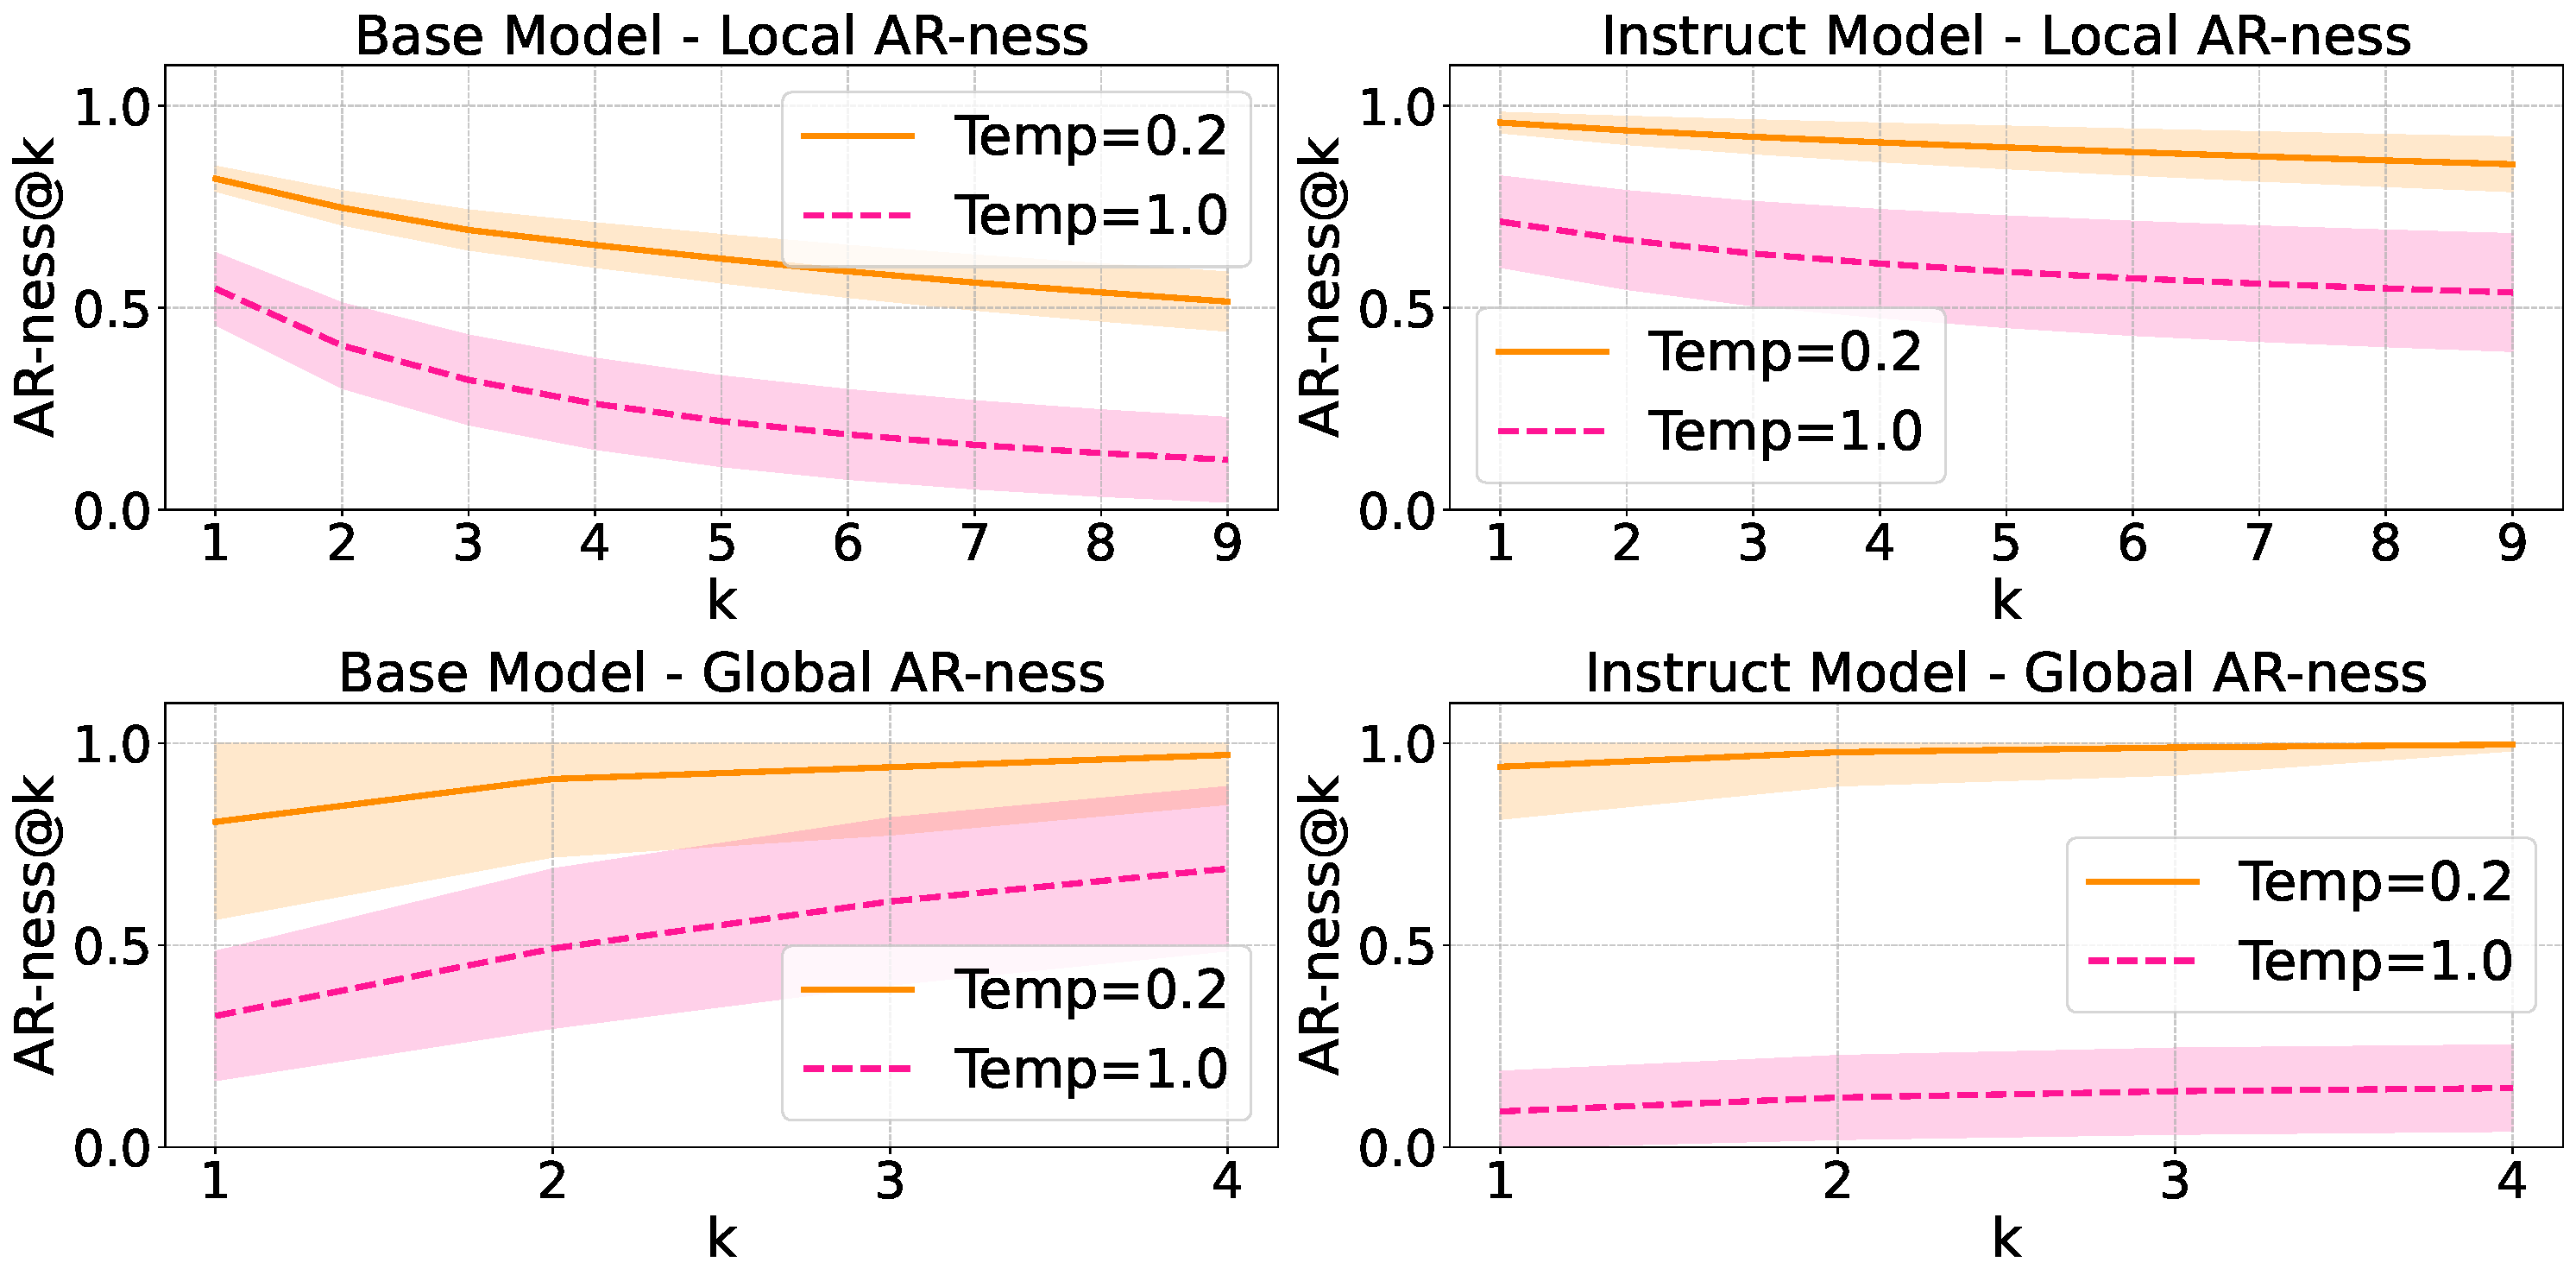
\includegraphics[width=\linewidth]{fig/ntpr-analysis-temp2.pdf}
  \end{subfigure}
  \hfill
  \begin{subfigure}[c]{0.48\textwidth}
    \centering
    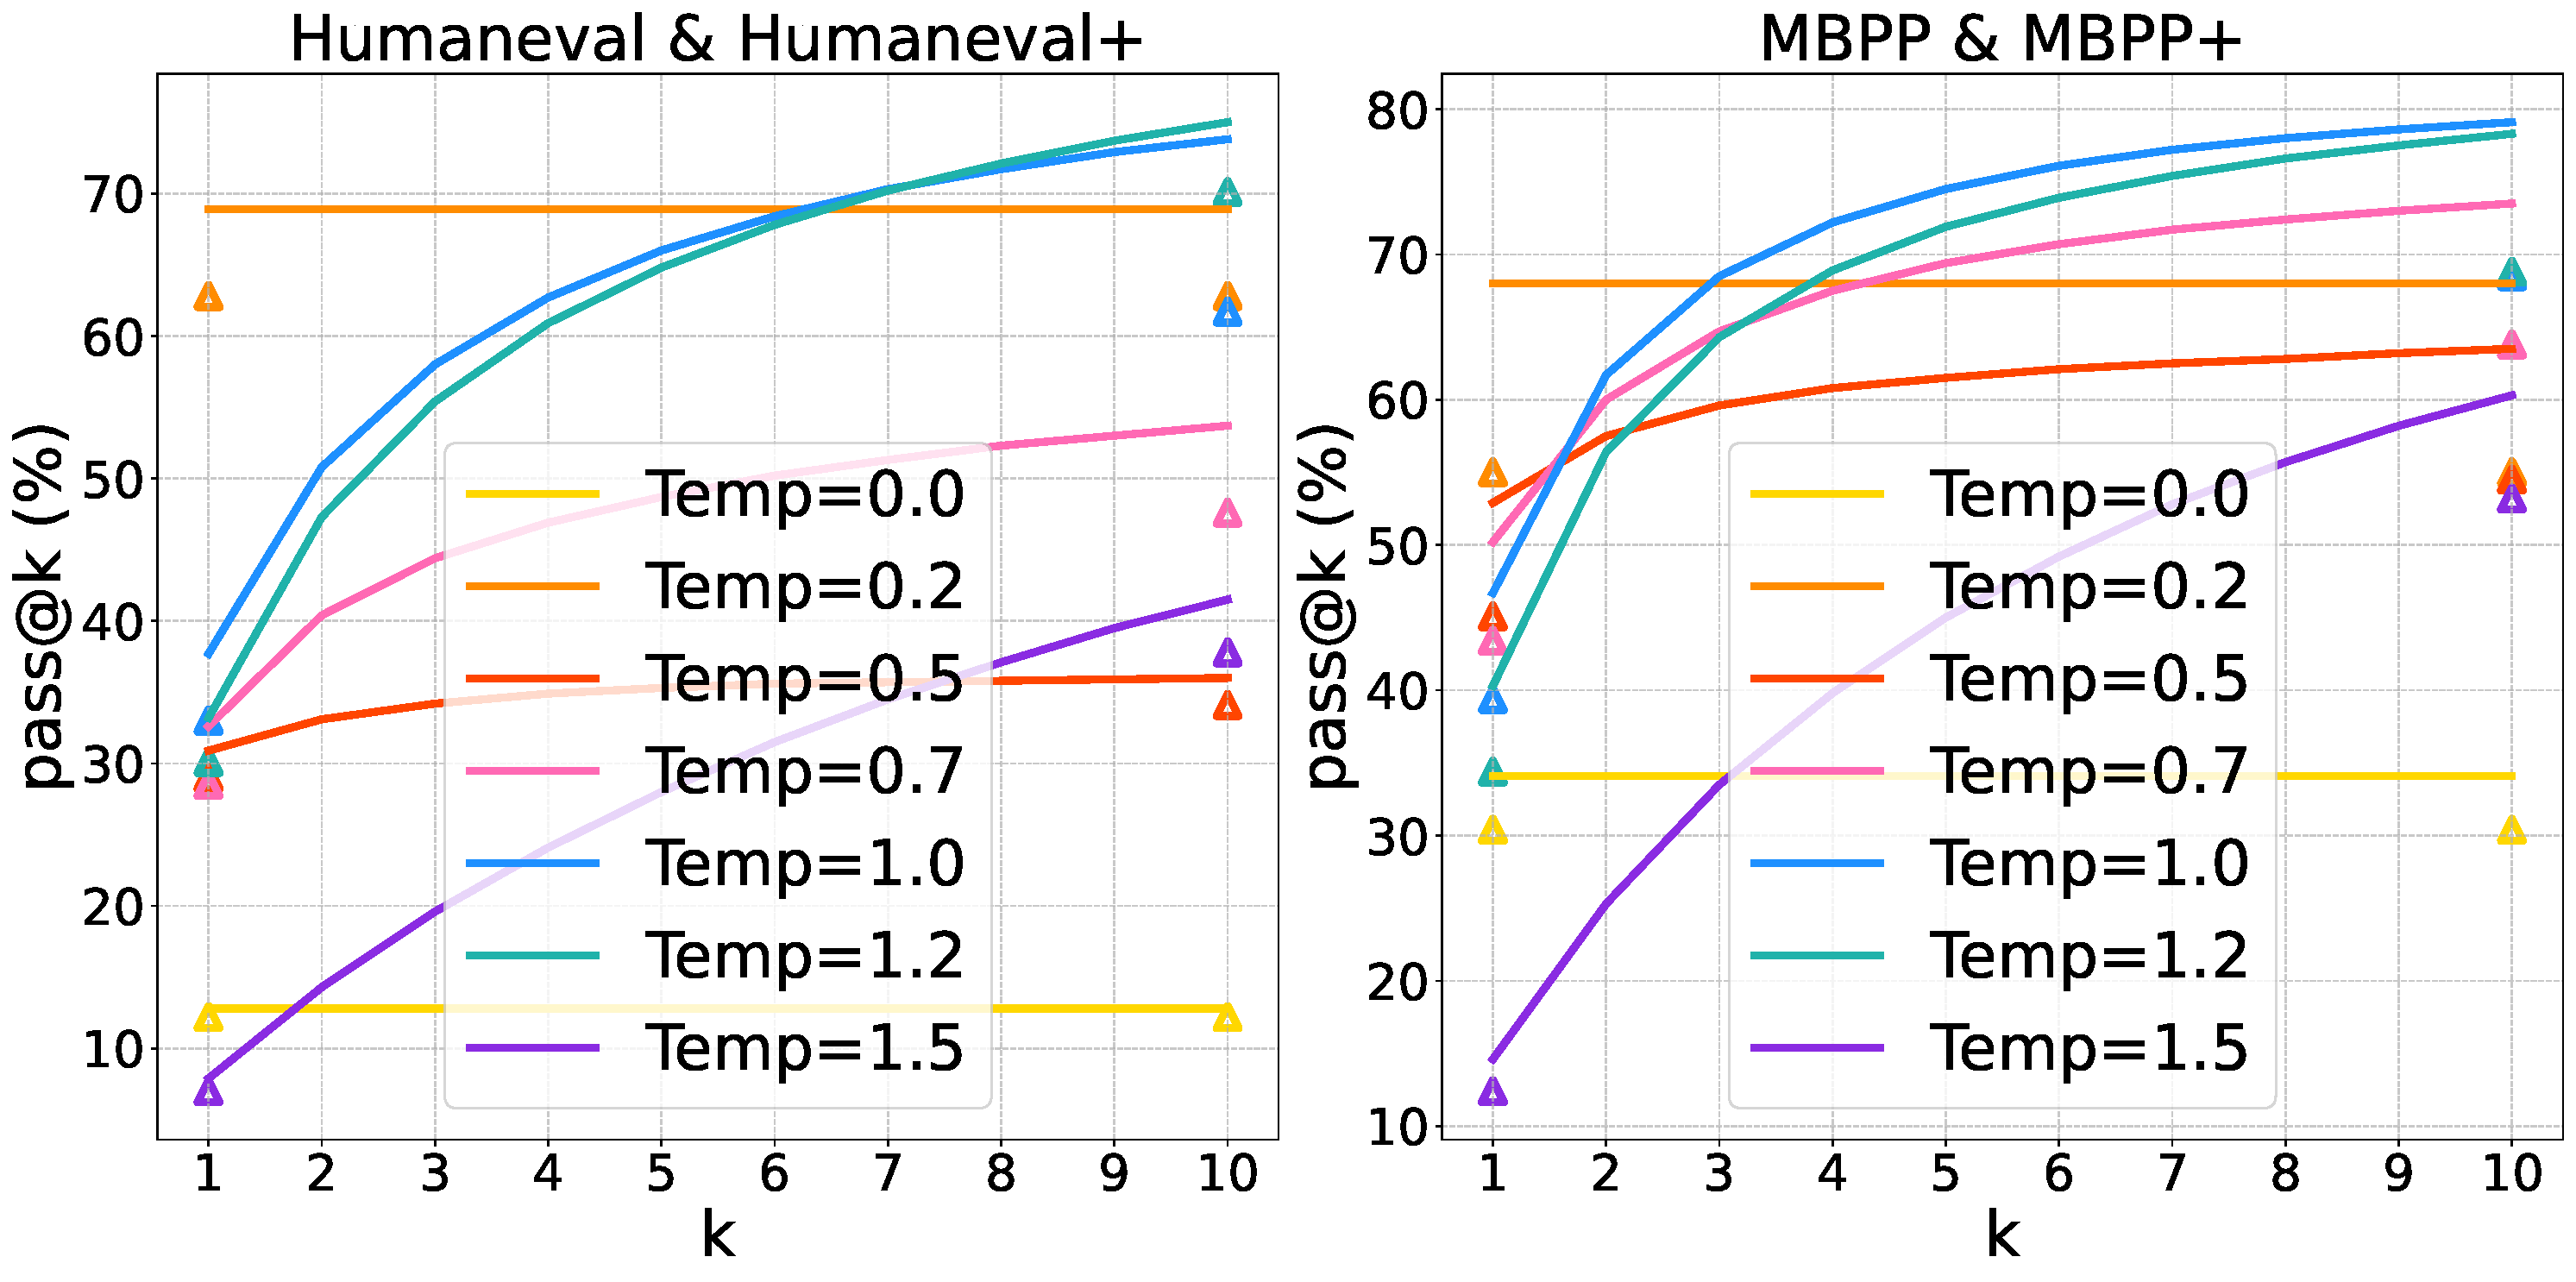
\includegraphics[width=\linewidth]{fig/temperature-analysis.pdf}
  \end{subfigure}
  \caption{Affects of different sampling temperatures. \textbf{Left}: For base model and instruct model, changing temperature affects the AR-ness on HumanEval. \textbf{Right}: pass@k curves are different for different temperatures, where triangles refer to score for plus version of each task.}
  \label{fig:diverse}
\end{figure}
\subsection{Generation Diversity}
\label{sec:gen-diver}
\begin{wrapfigure}{r}{0.4\textwidth}
  \centering
  \vspace{-13mm}
  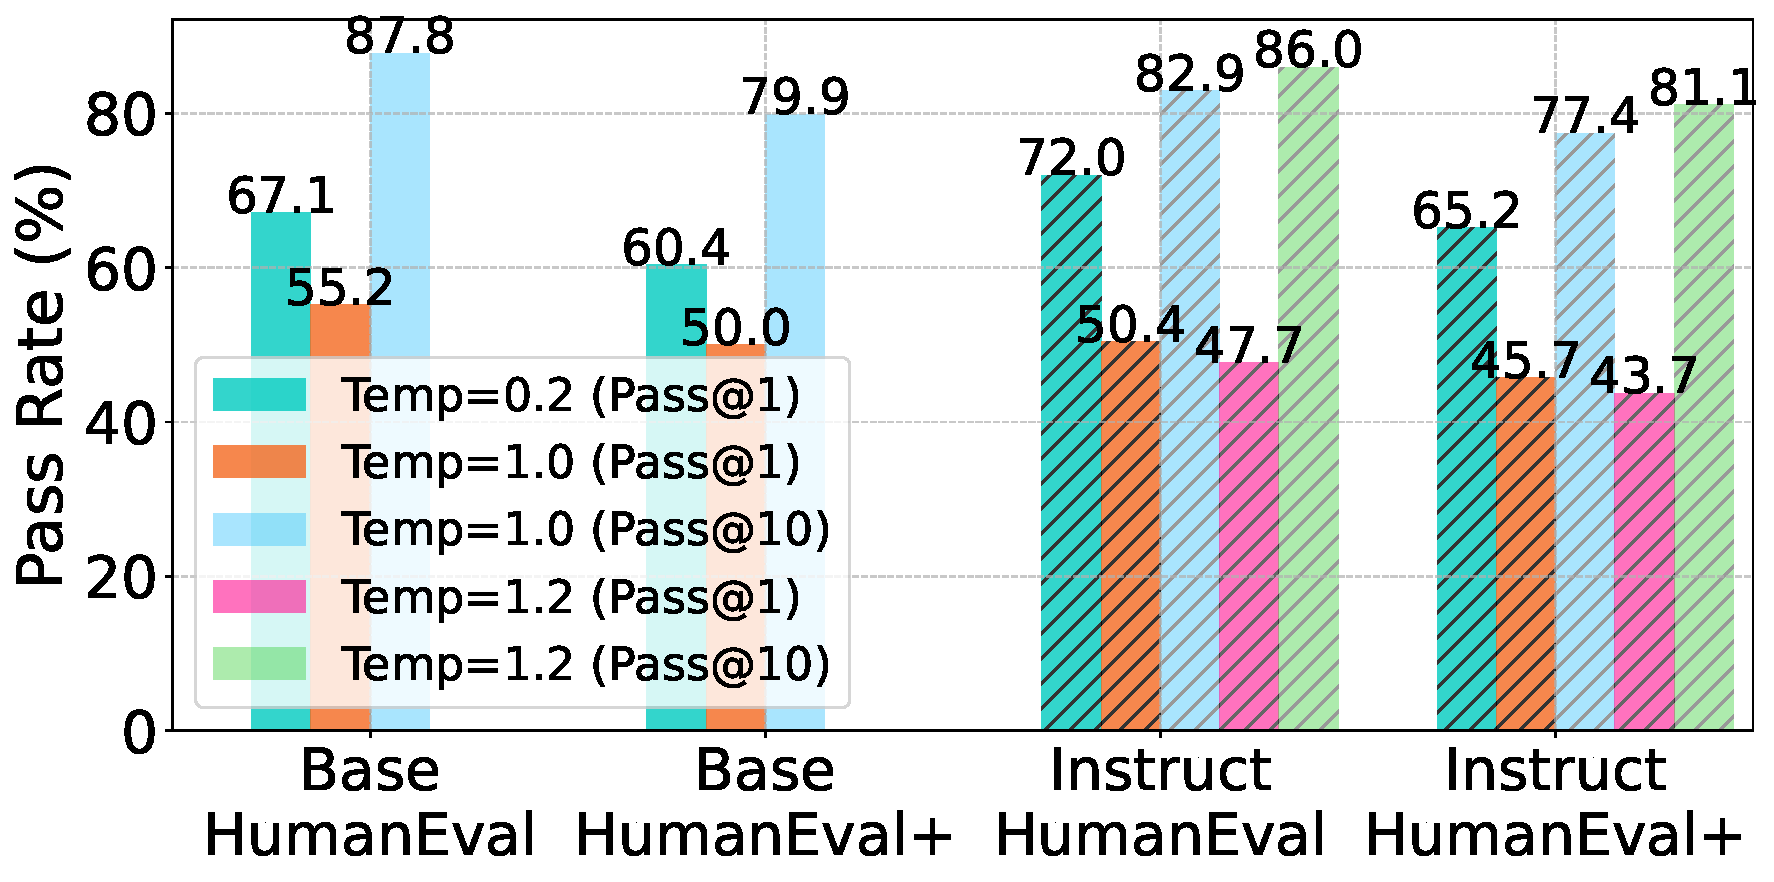
\includegraphics[width=0.4\textwidth]{fig/pass-rates-analysis.pdf}
  \caption{Pass@$k$ scores for different models and temperatures.}
  \label{fig:passk}
  \vspace{-2mm}
\end{wrapfigure}
Post-training studies on AR LLMs~\citep{yue2025does} show that an RL model's reasoning paths are bounded by the base model's pass@k sampling capabilities. 
Therefore, we examine generation diversity with pass@$k$ accuracy in dLLMs. 
As Figure~\ref{fig:diverse} (right) and Figure~\ref{fig:passk} illustrate, for both the base and instruct versions of DiffuCoder, a low temperature yields high pass@1 but little growth in pass@$k$, indicating that the samples lack diversity. 
By increasing the temperature to a suitable range (\textit{e.g.}, $1.0$ to $1.2$), pass@$k$ rises significantly, revealing a latent capability in the model. 
In many RL settings~\citep{bercovich2025llama,liu2025prorl}, the model must be able to sample diverse responses during rollouts before RL can reinforce pass@1 accuracy. 
The promising pass@$k$ curves of DiffuCoder indicate substantial room for improvement through RL, motivating the design of our coupled-GRPO algorithm (\S\ref{sec:grpo}).
Moreover, a higher temperature also substantially lowers AR-ness, as shown in Figure~\ref{fig:diverse} (left) and Figure~\ref{fig:teaser}(a), meaning the model generates tokens in a more random order, which operates differently from AR models. 
\textbf{In AR models, temperature only affects token selection, while in dLLMs it influences both token selection and their generated order.} A visualization of the decoding process from real samples is provided in Appx.~\ref{sec:appx:samples}. 